% GNUPLOT: LaTeX picture with Postscript
\begingroup
  \makeatletter
  \providecommand\color[2][]{%
    \GenericError{(gnuplot) \space\space\space\@spaces}{%
      Package color not loaded in conjunction with
      terminal option `colourtext'%
    }{See the gnuplot documentation for explanation.%
    }{Either use 'blacktext' in gnuplot or load the package
      color.sty in LaTeX.}%
    \renewcommand\color[2][]{}%
  }%
  \providecommand\includegraphics[2][]{%
    \GenericError{(gnuplot) \space\space\space\@spaces}{%
      Package graphicx or graphics not loaded%
    }{See the gnuplot documentation for explanation.%
    }{The gnuplot epslatex terminal needs graphicx.sty or graphics.sty.}%
    \renewcommand\includegraphics[2][]{}%
  }%
  \providecommand\rotatebox[2]{#2}%
  \@ifundefined{ifGPcolor}{%
    \newif\ifGPcolor
    \GPcolorfalse
  }{}%
  \@ifundefined{ifGPblacktext}{%
    \newif\ifGPblacktext
    \GPblacktexttrue
  }{}%
  % define a \g@addto@macro without @ in the name:
  \let\gplgaddtomacro\g@addto@macro
  % define empty templates for all commands taking text:
  \gdef\gplbacktext{}%
  \gdef\gplfronttext{}%
  \makeatother
  \ifGPblacktext
    % no textcolor at all
    \def\colorrgb#1{}%
    \def\colorgray#1{}%
  \else
    % gray or color?
    \ifGPcolor
      \def\colorrgb#1{\color[rgb]{#1}}%
      \def\colorgray#1{\color[gray]{#1}}%
      \expandafter\def\csname LTw\endcsname{\color{white}}%
      \expandafter\def\csname LTb\endcsname{\color{black}}%
      \expandafter\def\csname LTa\endcsname{\color{black}}%
      \expandafter\def\csname LT0\endcsname{\color[rgb]{1,0,0}}%
      \expandafter\def\csname LT1\endcsname{\color[rgb]{0,1,0}}%
      \expandafter\def\csname LT2\endcsname{\color[rgb]{0,0,1}}%
      \expandafter\def\csname LT3\endcsname{\color[rgb]{1,0,1}}%
      \expandafter\def\csname LT4\endcsname{\color[rgb]{0,1,1}}%
      \expandafter\def\csname LT5\endcsname{\color[rgb]{1,1,0}}%
      \expandafter\def\csname LT6\endcsname{\color[rgb]{0,0,0}}%
      \expandafter\def\csname LT7\endcsname{\color[rgb]{1,0.3,0}}%
      \expandafter\def\csname LT8\endcsname{\color[rgb]{0.5,0.5,0.5}}%
    \else
      % gray
      \def\colorrgb#1{\color{black}}%
      \def\colorgray#1{\color[gray]{#1}}%
      \expandafter\def\csname LTw\endcsname{\color{white}}%
      \expandafter\def\csname LTb\endcsname{\color{black}}%
      \expandafter\def\csname LTa\endcsname{\color{black}}%
      \expandafter\def\csname LT0\endcsname{\color{black}}%
      \expandafter\def\csname LT1\endcsname{\color{black}}%
      \expandafter\def\csname LT2\endcsname{\color{black}}%
      \expandafter\def\csname LT3\endcsname{\color{black}}%
      \expandafter\def\csname LT4\endcsname{\color{black}}%
      \expandafter\def\csname LT5\endcsname{\color{black}}%
      \expandafter\def\csname LT6\endcsname{\color{black}}%
      \expandafter\def\csname LT7\endcsname{\color{black}}%
      \expandafter\def\csname LT8\endcsname{\color{black}}%
    \fi
  \fi
    \setlength{\unitlength}{0.0500bp}%
    \ifx\gptboxheight\undefined%
      \newlength{\gptboxheight}%
      \newlength{\gptboxwidth}%
      \newsavebox{\gptboxtext}%
    \fi%
    \setlength{\fboxrule}{0.5pt}%
    \setlength{\fboxsep}{1pt}%
\begin{picture}(7200.00,5040.00)%
    \gplgaddtomacro\gplbacktext{%
      \csname LTb\endcsname%%
      \put(588,3198){\makebox(0,0)[r]{\strut{}0.00}}%
      \csname LTb\endcsname%%
      \put(588,3893){\makebox(0,0)[r]{\strut{}0.35}}%
      \csname LTb\endcsname%%
      \put(588,4587){\makebox(0,0)[r]{\strut{}0.70}}%
      \csname LTb\endcsname%%
      \put(919,2879){\makebox(0,0){\strut{}$0$}}%
      \csname LTb\endcsname%%
      \put(1716,2879){\makebox(0,0){\strut{}$2$}}%
      \csname LTb\endcsname%%
      \put(2513,2879){\makebox(0,0){\strut{}$4$}}%
      \csname LTb\endcsname%%
      \put(3309,2879){\makebox(0,0){\strut{}$6$}}%
      \csname LTb\endcsname%%
      \put(4106,2879){\makebox(0,0){\strut{}$8$}}%
      \csname LTb\endcsname%%
      \put(4903,2879){\makebox(0,0){\strut{}$10$}}%
      \csname LTb\endcsname%%
      \put(5699,2879){\makebox(0,0){\strut{}$12$}}%
      \csname LTb\endcsname%%
      \put(6496,2879){\makebox(0,0){\strut{}$14$}}%
    }%
    \gplgaddtomacro\gplfronttext{%
      \csname LTb\endcsname%%
      \put(-50,3892){\rotatebox{-270}{\makebox(0,0){\strut{}$\alpha_{\rm central}$}}}%
      \put(3707,569){\makebox(0,0){\strut{}$t$}}%
      \csname LTb\endcsname%%
      \put(5708,4458){\makebox(0,0)[r]{\strut{}$\eta = 0.01591203885327$}}%
      \csname LTb\endcsname%%
      \put(5708,4238){\makebox(0,0)[r]{\strut{}$\eta = 0.01591203885328$}}%
    }%
    \gplgaddtomacro\gplbacktext{%
      \csname LTb\endcsname%%
      \put(3935,1273){\makebox(0,0)[r]{\strut{}0.0}}%
      \csname LTb\endcsname%%
      \put(3935,1802){\makebox(0,0)[r]{\strut{}$0.1$}}%
      \csname LTb\endcsname%%
      \put(3935,2331){\makebox(0,0)[r]{\strut{}$0.2$}}%
      \csname LTb\endcsname%%
      \put(4442,788){\makebox(0,0){\strut{}13.00}}%
      \csname LTb\endcsname%%
      \put(5381,788){\makebox(0,0){\strut{}$13.25$}}%
      \csname LTb\endcsname%%
      \put(6320,788){\makebox(0,0){\strut{}13.50}}%
    }%
    \gplgaddtomacro\gplfronttext{%
    }%
    \gplgaddtomacro\gplbacktext{%
      \csname LTb\endcsname%%
      \put(588,1235){\makebox(0,0)[r]{\strut{}0.00}}%
      \csname LTb\endcsname%%
      \put(588,1802){\makebox(0,0)[r]{\strut{}$0.05$}}%
      \csname LTb\endcsname%%
      \put(588,2368){\makebox(0,0)[r]{\strut{}0.10}}%
      \csname LTb\endcsname%%
      \put(1245,788){\makebox(0,0){\strut{}13.470}}%
      \csname LTb\endcsname%%
      \put(2033,788){\makebox(0,0){\strut{}$13.485$}}%
      \csname LTb\endcsname%%
      \put(2822,788){\makebox(0,0){\strut{}13.500}}%
    }%
    \gplgaddtomacro\gplfronttext{%
    }%
    \gplbacktext
    \put(0,0){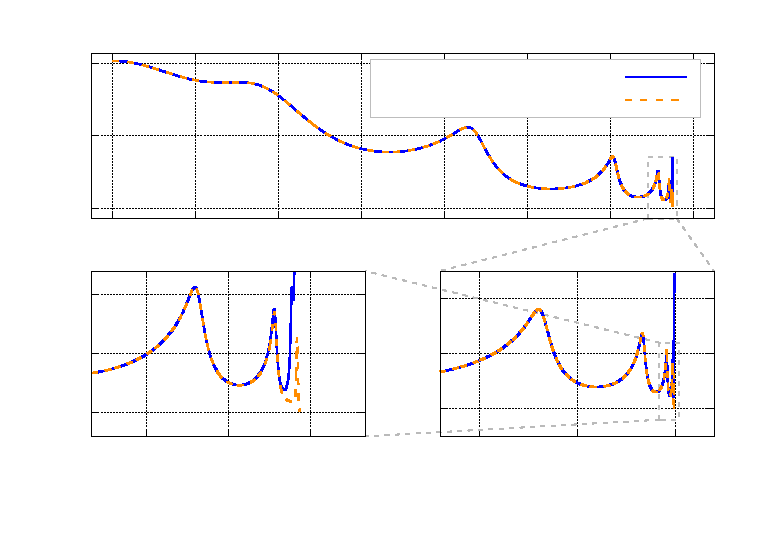
\includegraphics{resources/critical_lapse_best_v2}}%
    \gplfronttext
  \end{picture}%
\endgroup
